\documentclass[12pt]{article}
\usepackage{graphicx} % Required for inserting images
\usepackage{mathtools}
\usepackage{amsmath}
\usepackage{gvv-book}
\usepackage{gvv}
\usepackage[shortlabels]{enumitem}
\usepackage{multicol}

\title{\textbf{12.434}}
\author{\textbf{EE25BTECH11004 - Aditya Appana}}
\date{October 12, 2025}
\renewcommand{\labelenumi}{\Alph{enumi})}
\begin{document}

\maketitle

\section*{Question}
The two sides of a parallelogram are given by the vectors $\vec{A}= 2\hat{i} - 3\hat{j}$ and $\vec{B} = 3\hat{i} + 2\hat{j}.$
The area of the parallelogram is:
\section*{Solution}
Let:
\begin{align}
    \vec{a} = \myvec{2\\-3\\0}\\
    \vec{b} = \myvec{3\\2\\0}
\end{align}\\
The area of the parallelogram can be expressed as:
\begin{align}
\vec{a}\times\vec{b}=
\myvec{|\vec{A_{23}} \vec{B_{23}}| \\ |\vec{A_{31}}   \vec{B_{31}}| \\ |\vec{A_{12}} \vec{B_{12}}| }
\end{align}
Substituting values:
\begin{align}
   \vec{a}\times\vec{b}= \myvec{0\\0\\13}
\end{align}
Therefore, the area of the parallelogram is:
\begin{align}
\norm{\vec{a}\times\vec{b}}  = 13
\end{align}
It can be seen that $\vec{a}$ and $\vec{b}$ are orthogonal, and $\norm{\vec{a}} = \norm{\vec{b}}$, therefore they form the sides of a square.\\
Therefore the area can also be calculated as:
\begin{align}
    {\norm{\vec{a}}}^2 = {\sqrt{13}}^2 = 13
\end{align}

\begin{figure}[H]
    \centering
    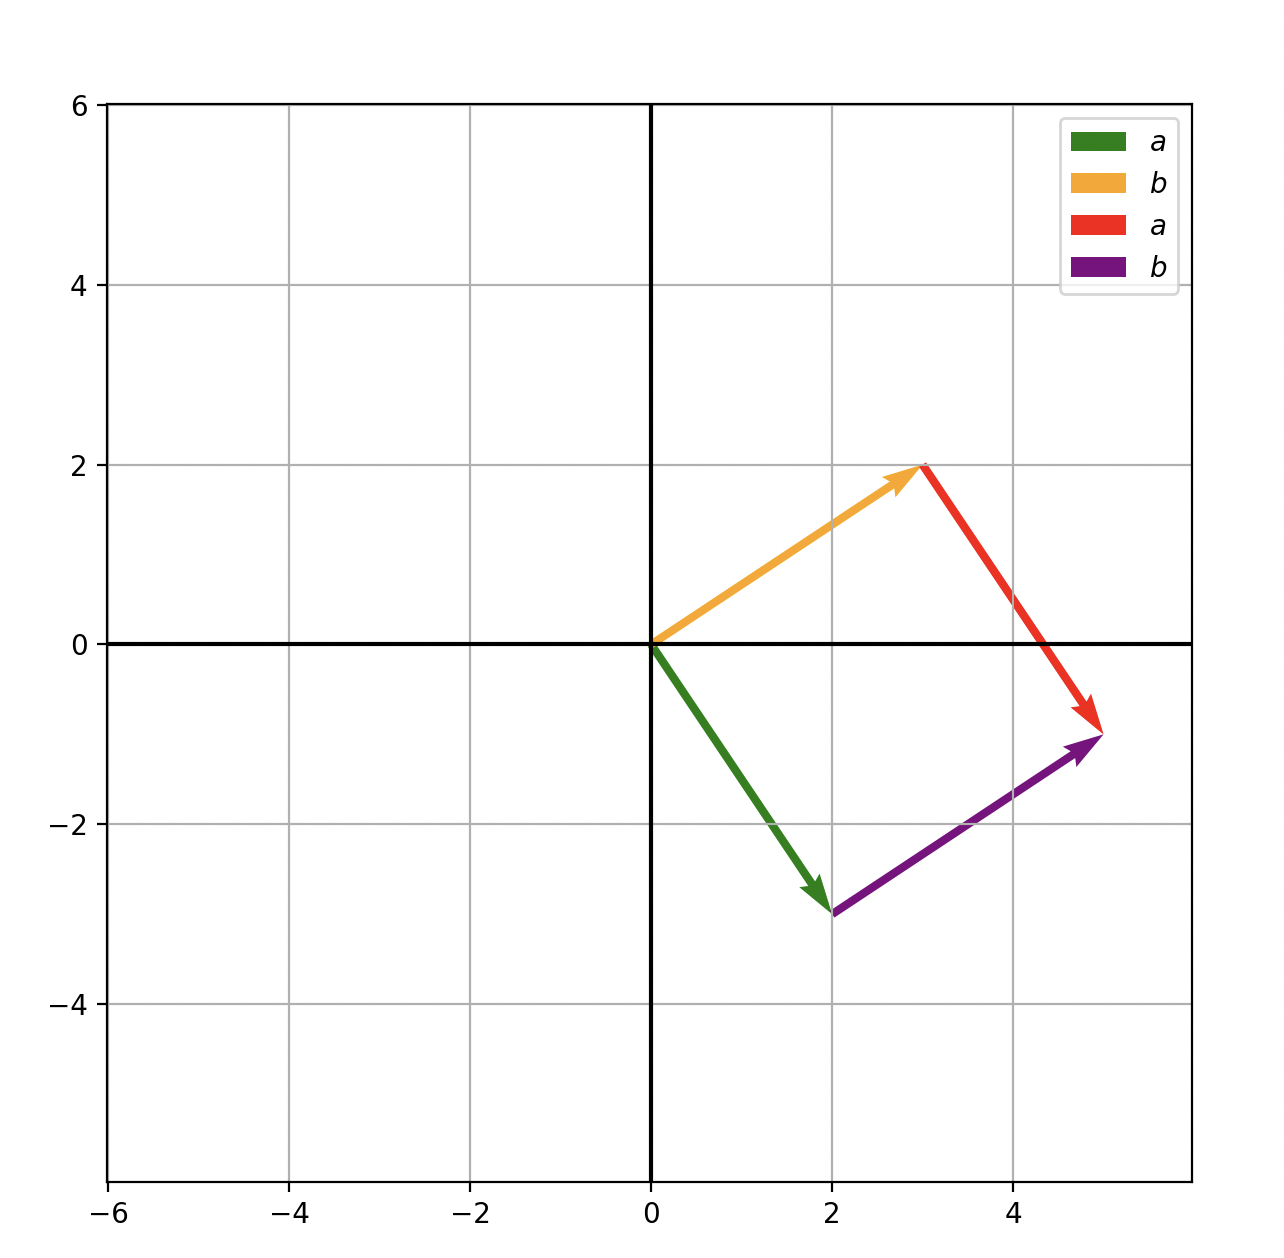
\includegraphics[width=0.7\columnwidth]{Figs/12434.png}
    \caption{Plot}
    \label{fig:placeholder}
\end{figure}\\

\end{document}
